% !TEX encoding = UTF-8 Unicode
%!TEX root = ../Main/thesis.tex
% !TEX spellcheck = en-US
%%=========================================
\documentclass[../Main/thesis.tex]{subfiles}
\begin{document}
\chapter{Second Iteration  - First prototype}
\label{ch:development-1}
This chapter describes the second iteration of the development.
In this iteration a prototype of both the Android application and the back-end was developed.
The iteration ended with a demonstration and test of the prototypes for Øygarden Fire and Rescue.

\section{Android application}
The goal for this iteration was to implement the Bluetooth data collecting functionality, and the possibility to upload a completed session to the server, using the design proposed in Chapter~\ref{ch:requirements}.

This version of the app is shown in Figure~\ref{fig:app-first-prototype}.
The first screen in the application (see Figure~\ref{fig:app-first-prototype-sessionlist}) contains a list of available sessions. 
Each session is represented with a name and the name of the person who is supposed to use that session.
When a smoke diver is getting ready for the exercise he chooses the appropriate session from the list which takes him to the next screen.

The second screen in the app (see Figure~\ref{fig:app-first-prototype-trackingactivity}) tells the user that the app is not currently tracking and has a blue play-button and instructions telling the user to press the button to start the tracking.
When a user press the play-button a dialog-box is shown asking for confirmation that the user want to start the tracking. 
If the user confirms he is taken to the third screen (see Figure~\ref{fig:app-first-prototype-tracking}) and the app start searching for BLE-signals.
Every time the app receives a BLE-signal it stores the signal-strength, identifiers of the beacon transmitting the signal, data from the gyroscope and accelerometer in the phone, and a timestamp, as a datapoint in the current session.
When the user has finished the tracking and presses the stop-button a new dialog appears to confirm that the user want to end the tracking.
If the user confirms all the recorded data is uploaded to the server for processing, and a upload-dialog is shown (see Figure~\ref{fig:app-first-prototype-upload}.
After the uploading is finished the user is taken back to the list of available sessions.

\begin{figure}[h]
	\centering
	\begin{subfigure}{0.2\textwidth}
		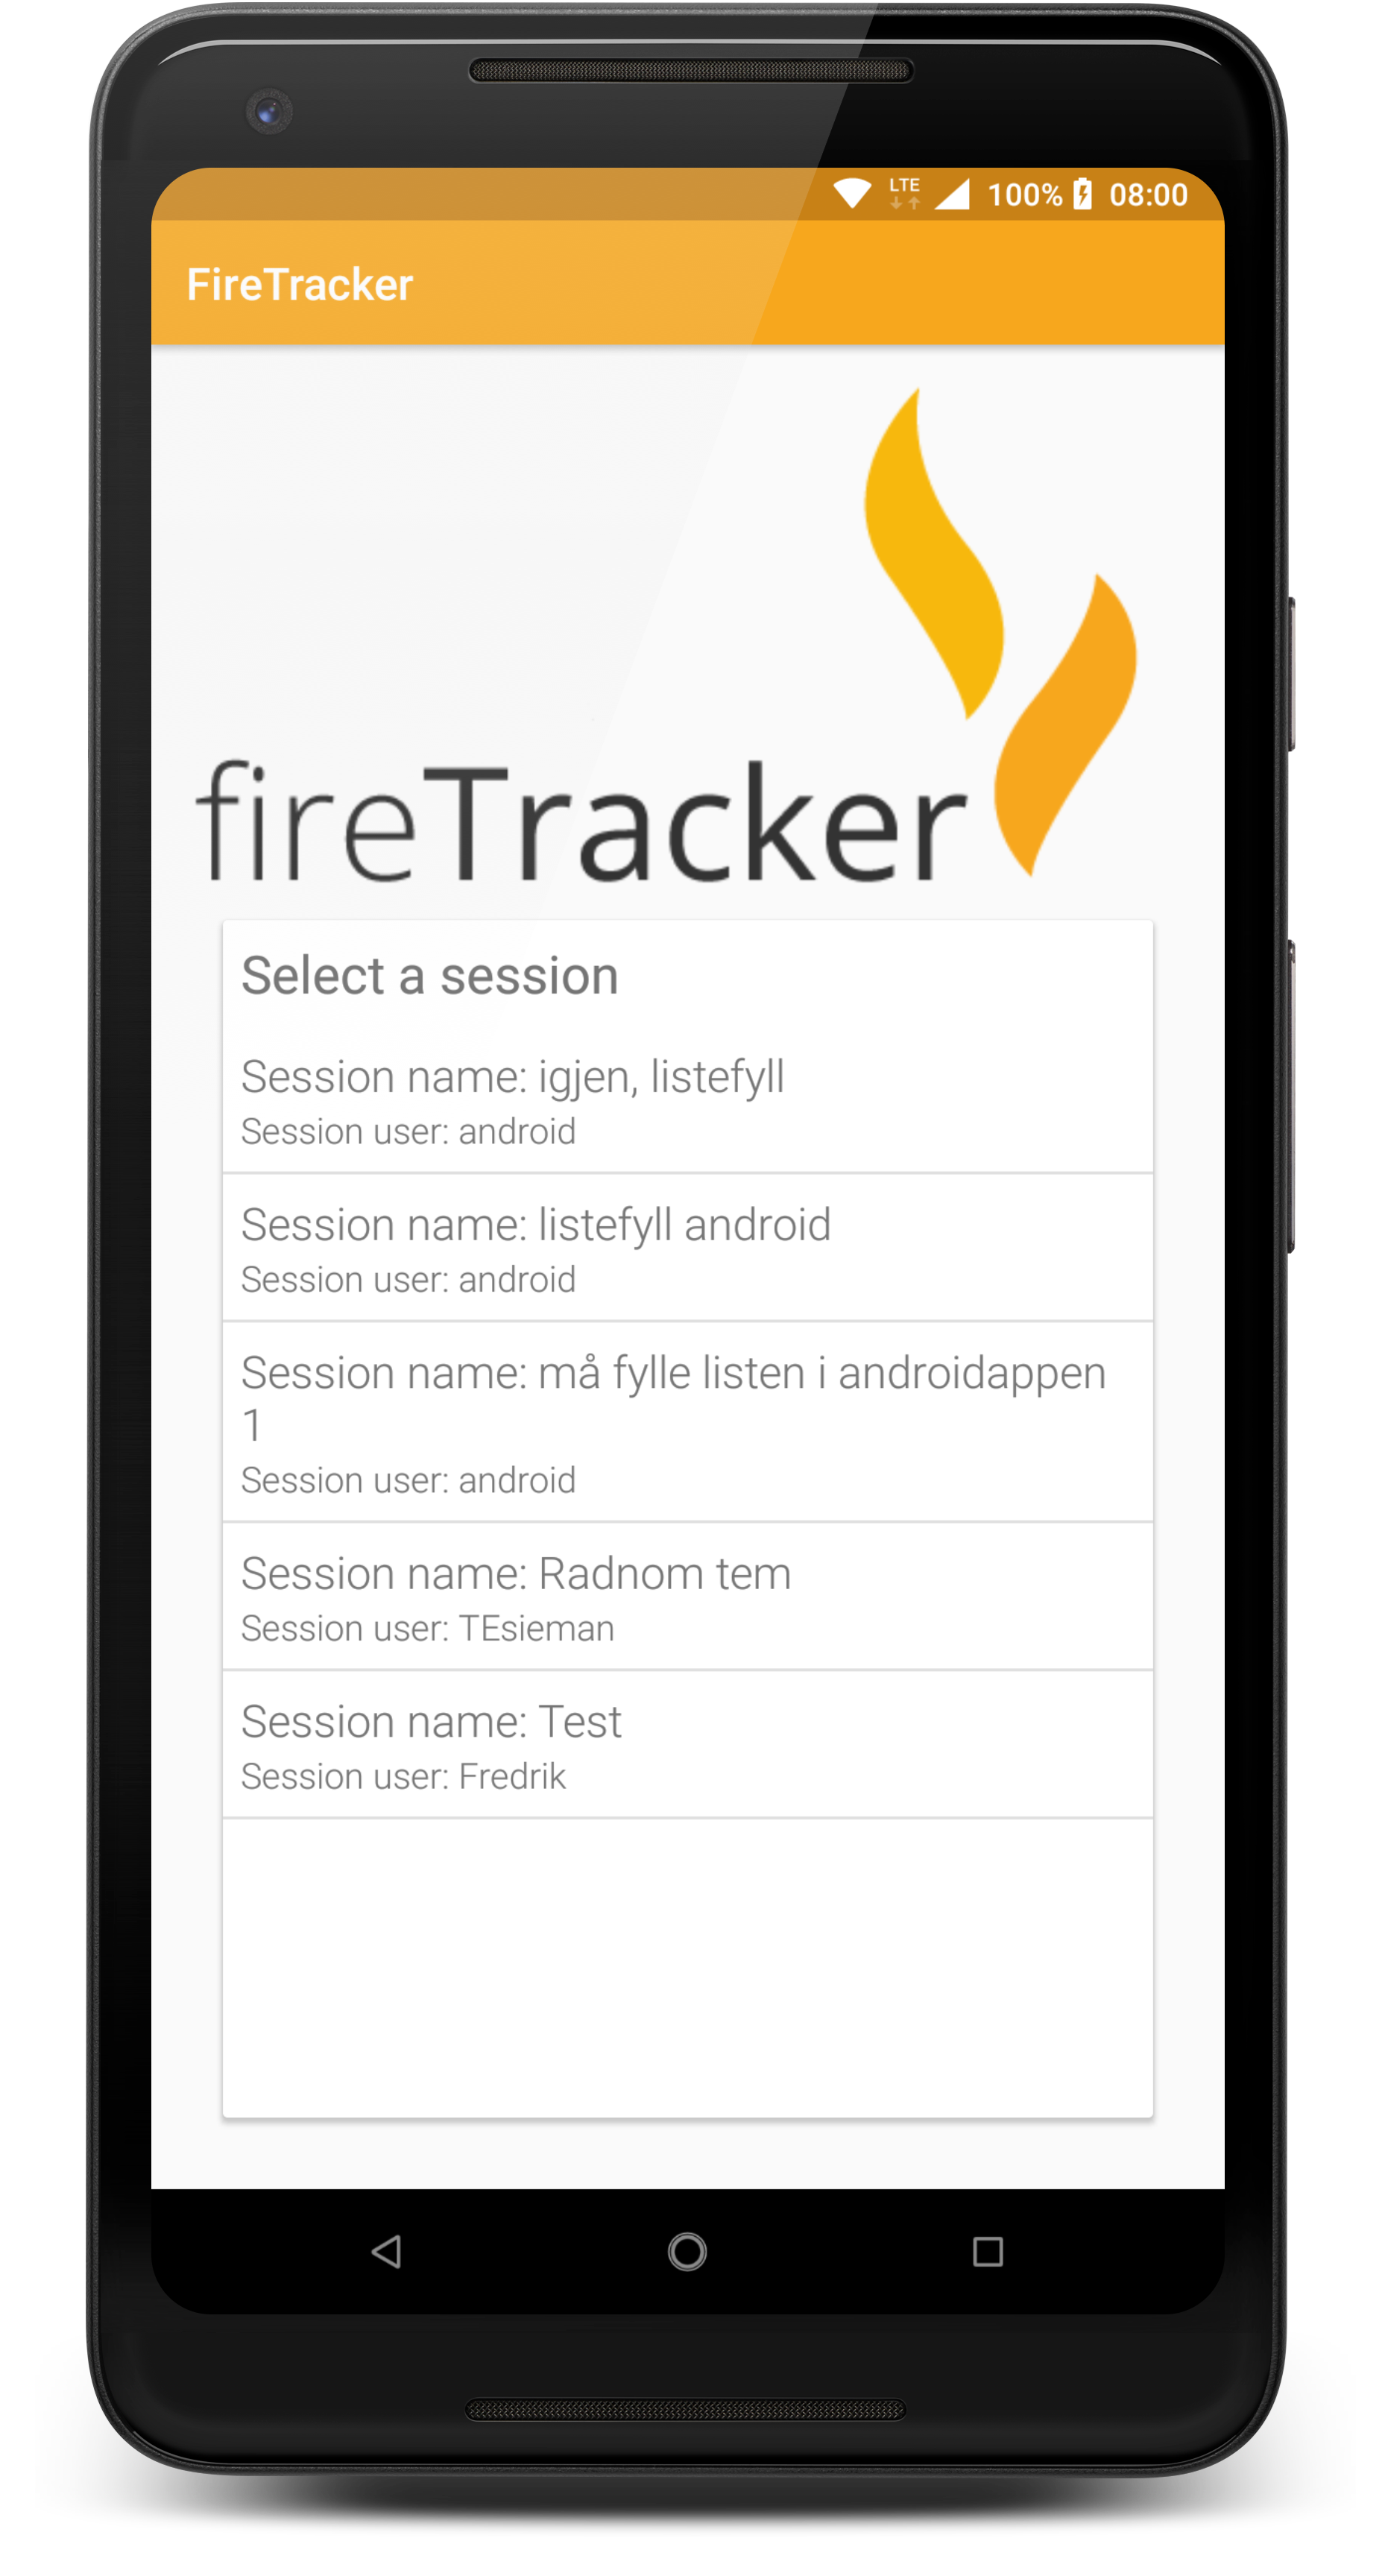
\includegraphics[width=\textwidth]{../fig/firetracker_app_old_1}
		\caption{List of sessions}
		\label{fig:app-first-prototype-sessionlist}
	\end{subfigure}
	\begin{subfigure}{0.2\textwidth}
		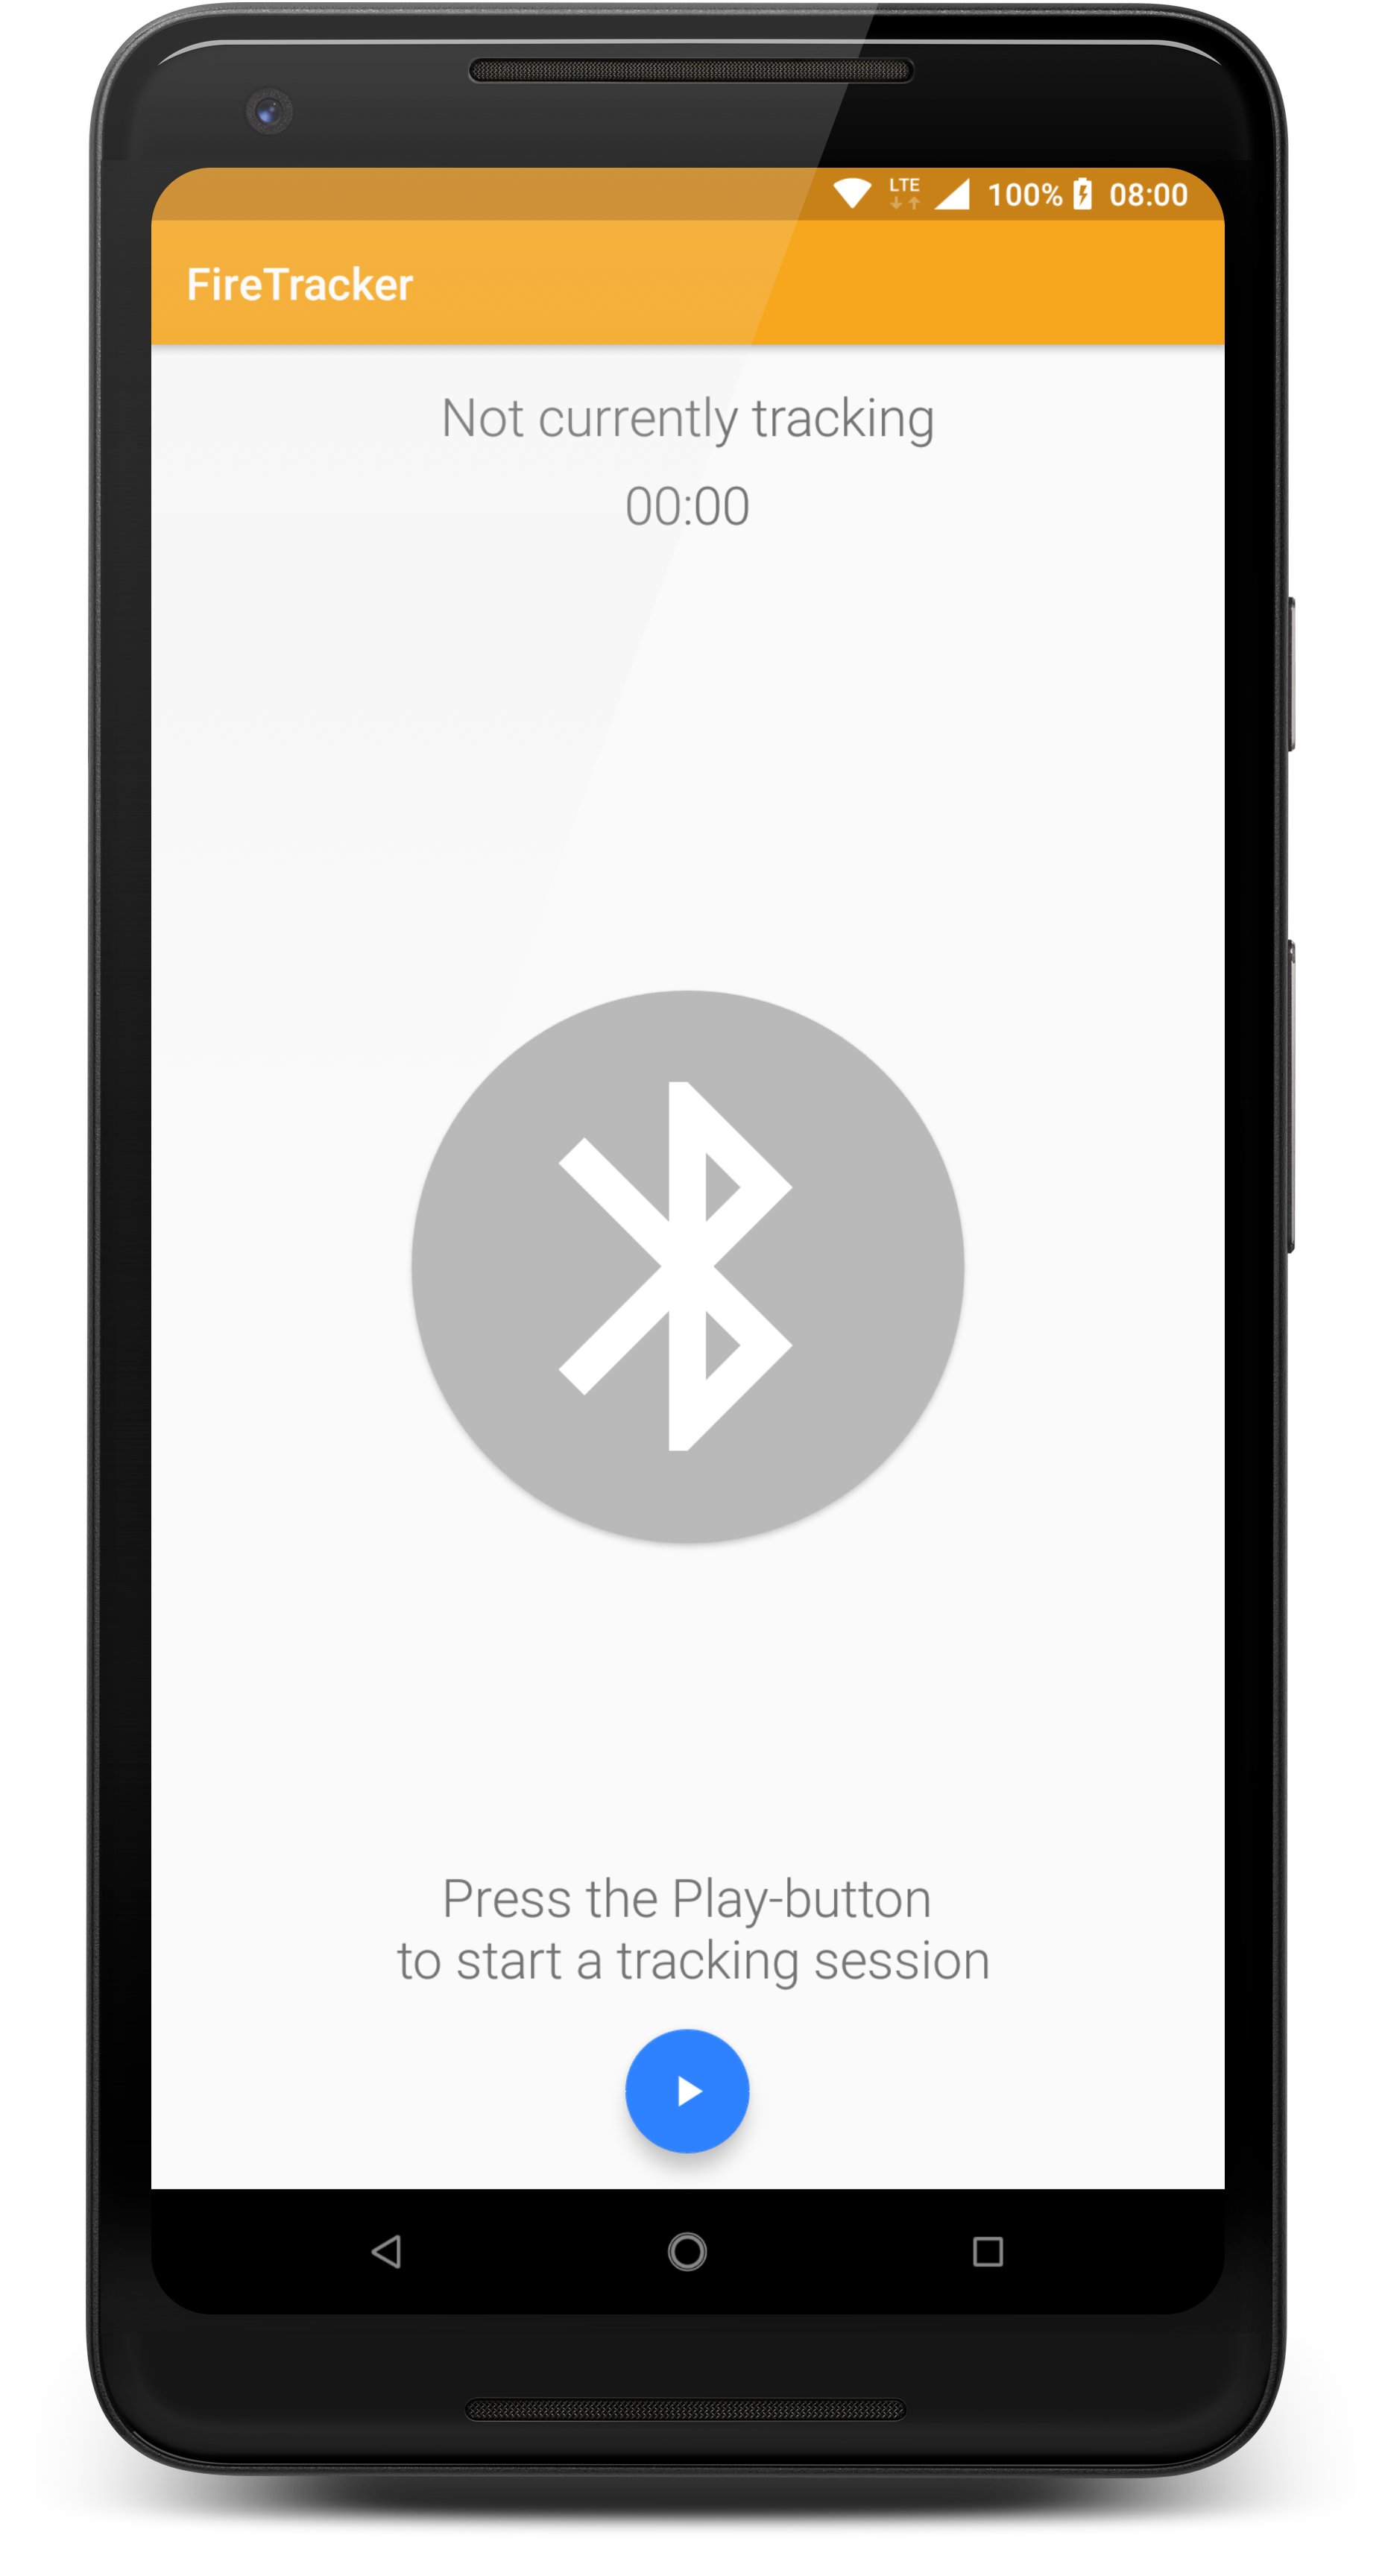
\includegraphics[width=\textwidth]{../fig/firetracker_app_old_2}
		\caption{Tracking activity}
		\label{fig:app-first-prototype-trackingactivity}
	\end{subfigure}
	\begin{subfigure}{0.2\textwidth}
		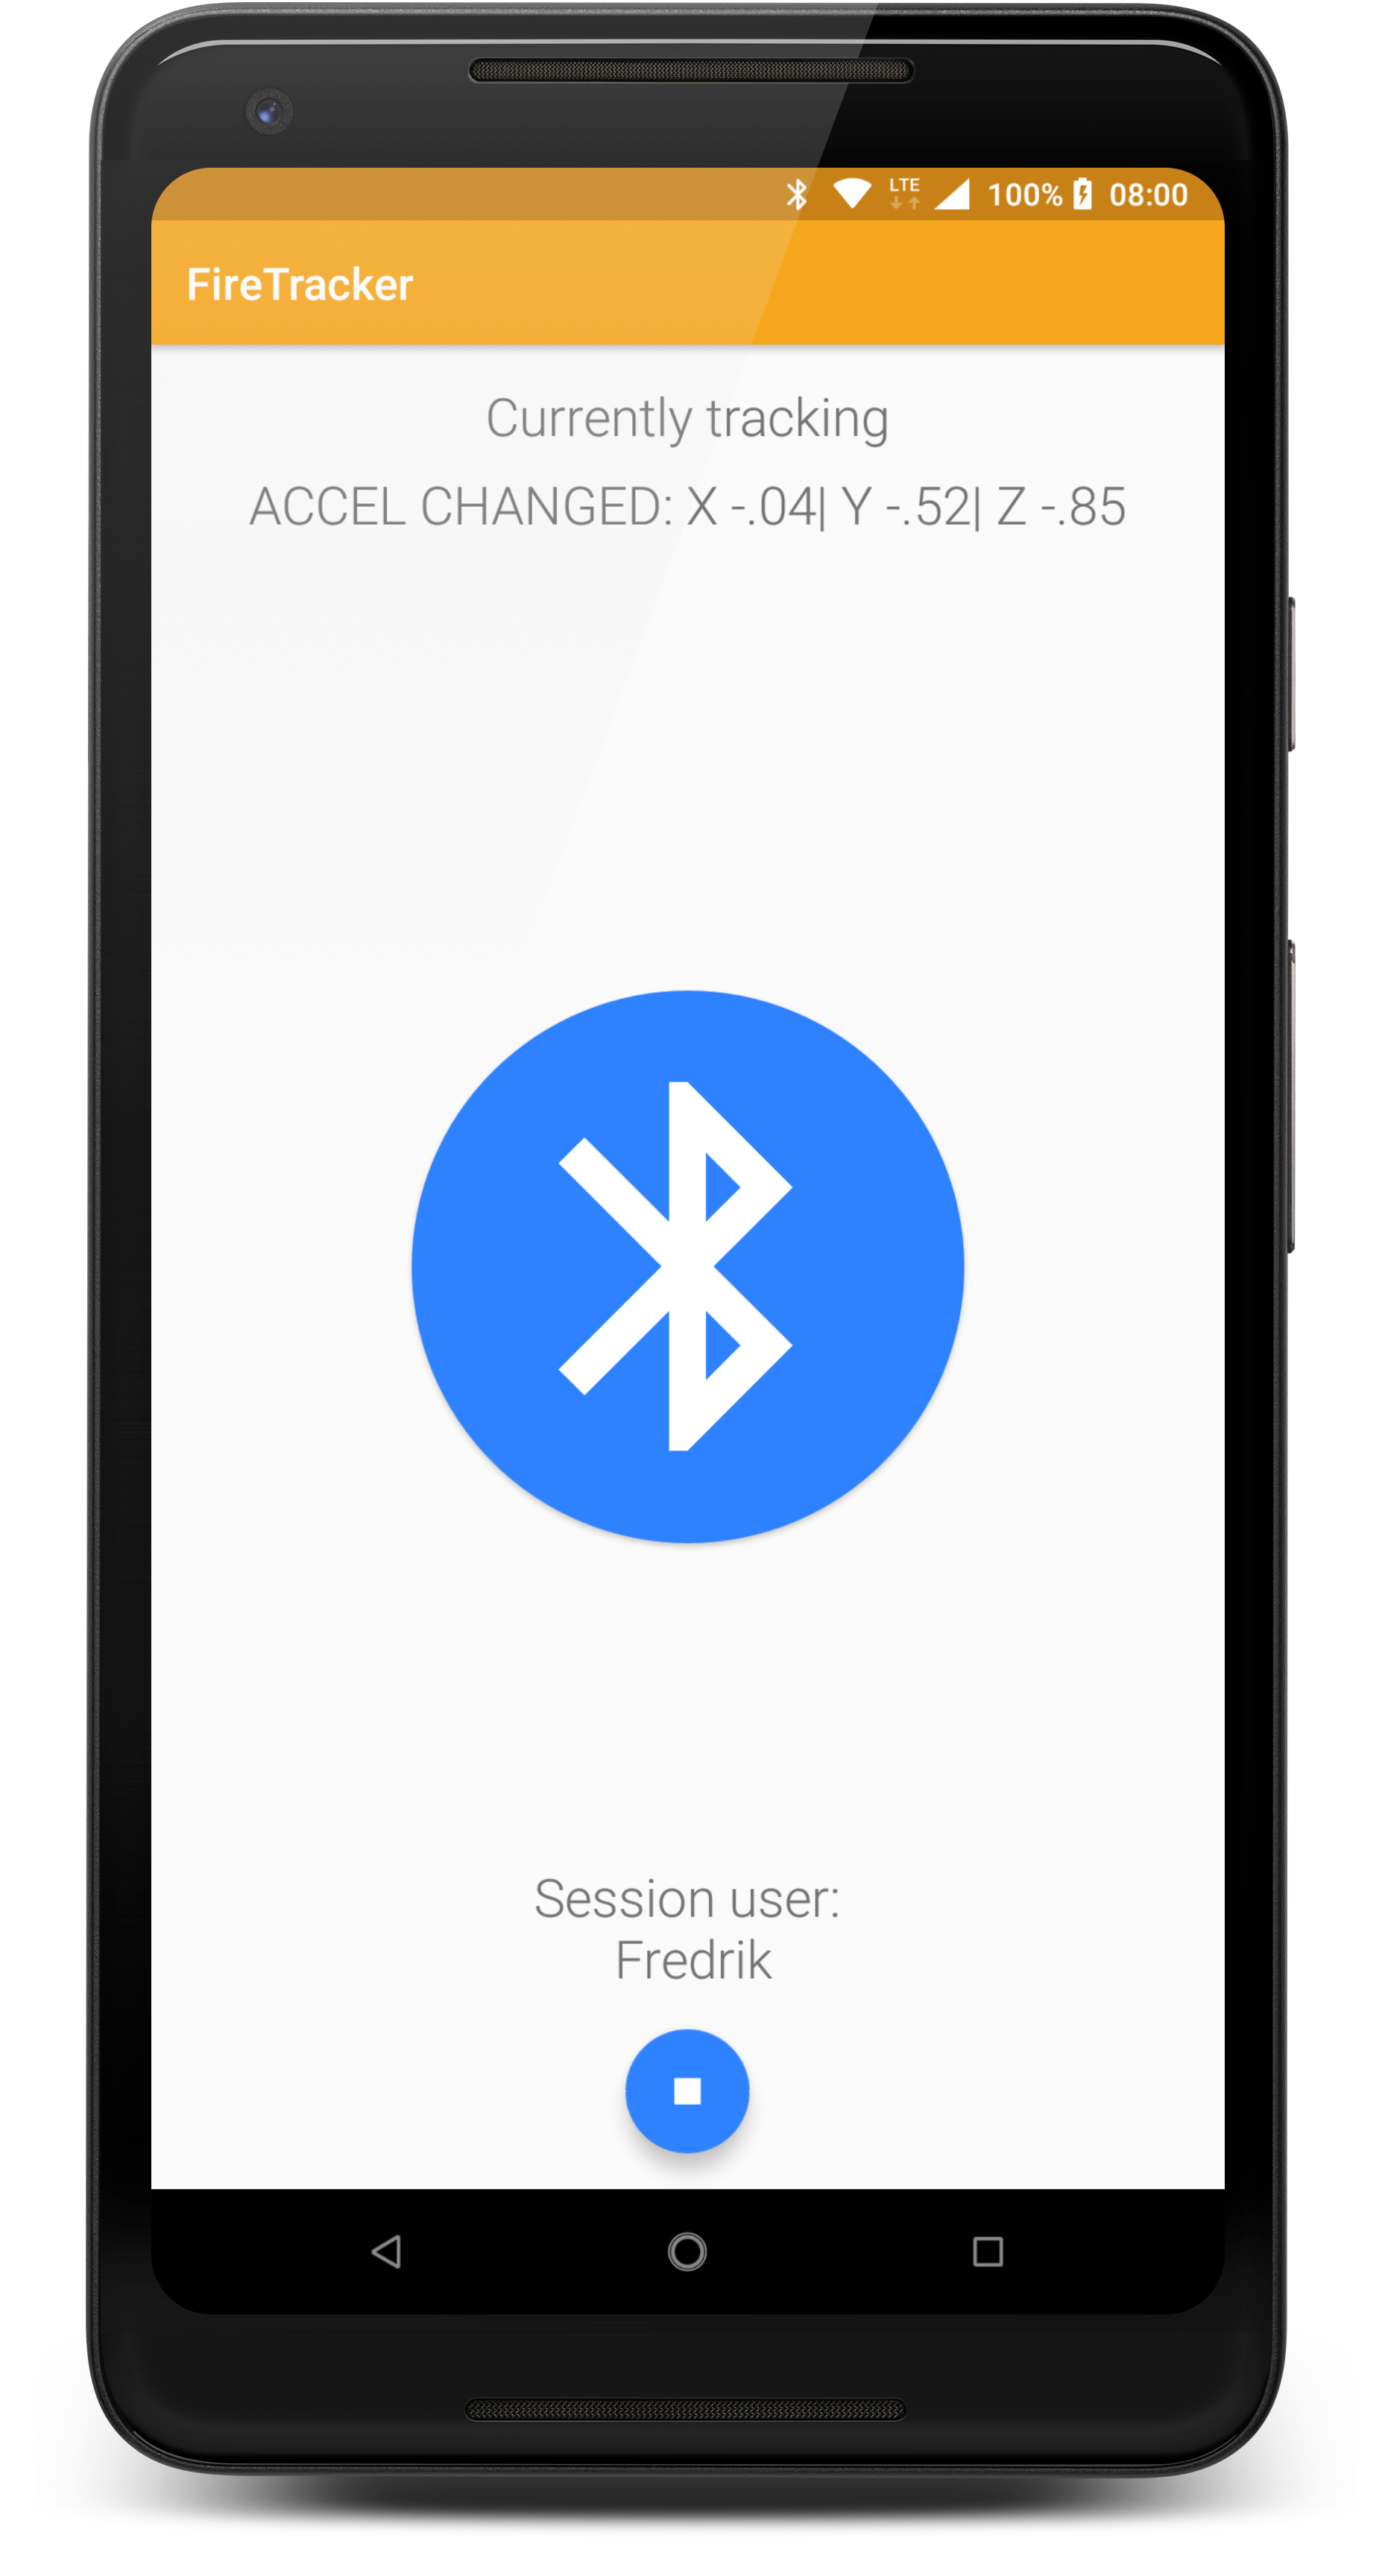
\includegraphics[width=\textwidth]{../fig/firetracker_app_old_3}
		\caption{Active tracking}
		\label{fig:app-first-prototype-tracking}
	\end{subfigure}
	\begin{subfigure}{0.2\textwidth}
		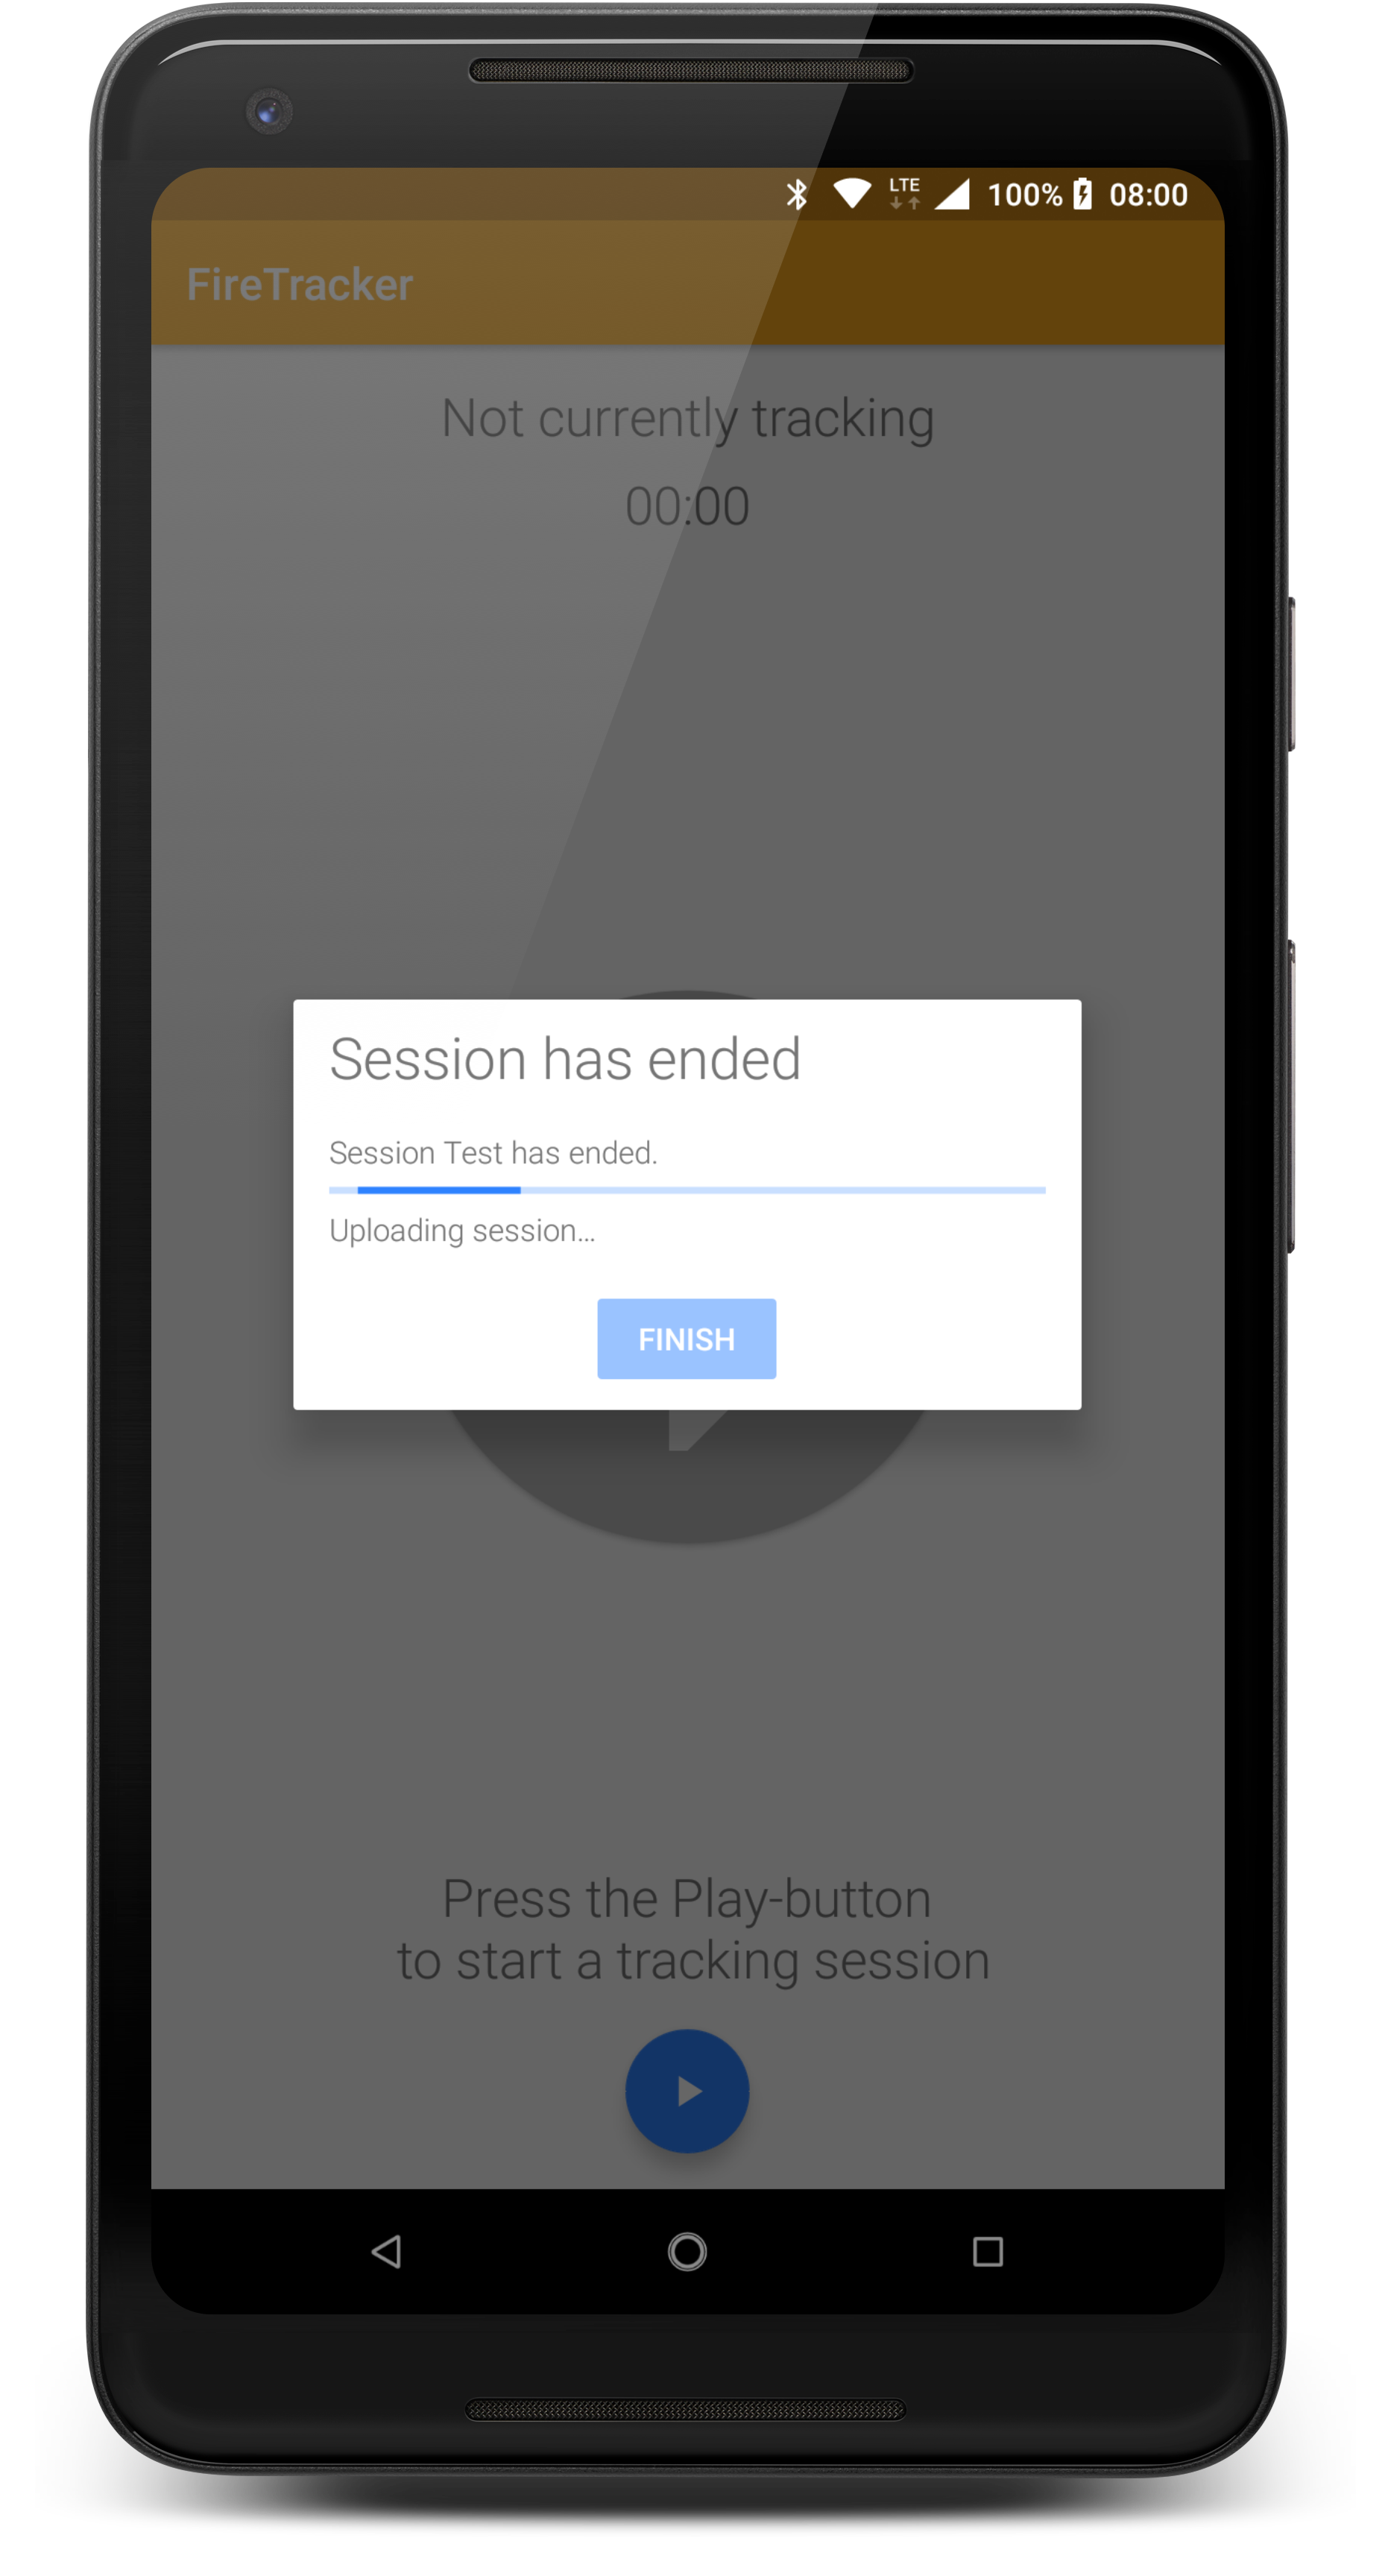
\includegraphics[width=\textwidth]{../fig/firetracker_app_old_4}
		\caption{Uploading data}
		\label{fig:app-first-prototype-upload}
	\end{subfigure}
	\caption{Screenshots of the Android application}
	\label{fig:app-first-prototype}
\end{figure}

\subsection*{Use of sensors}
In addition to tracking Bluetooth-data the app also records data from the built-in accelerometer and gyroscope in the smartphone.
The accelerometer was used to detect movement and create an estimate of how many steps the user takes during the tracking.
This information was then used to determine if the smoke diver was walking around or standing still within a location.

The gyroscope was used to collect information about the relative orientation of the smartphone. 
The intention was to use this data to determine the orientation of the smoke diver within the building, but it turned out that different devices had different zero positioning.
Therefore it was not possible to determine a consistent orientation across devices.
Instead the difference of orientation over a time interval was used to determine if the user rotating the device, and thereby rotating their head as the device. 

\section{Back-end}
The back-end of the FireTracker system consists of two parts.
A web-server that handles requests from the Android application and the exercise management tools and returns data to them
A part that processes the raw data from the Android app and outputs data about the locations and movements of the firefighters that can be used by the exercise management tool to create a visualization.
In this iteration the web-server functionality was implemented together with a basic processing algorithm.

\subsection{Web-server}
The web-server handles HTTP requests from the other components of the FireTracker system and stores data it receives in a database. 
It also fetches data from this database and return it to the Android app or the exercise management tool when they ask for data.
In this iteration a variety of endpoints were implemented allowing the creation of new sessions, retrieving a list of unprocessed or processed sessions, retrieving a single unprocessed or processed session, updating an unprocessed session, adding beacons and maps, and retrieving a list of beacons. 
An overview of all the endpoints is shown in Table~\ref{tab:endpoints-1}.

\begin{table}[h]
\caption{Web-server endpoints implemented in the second iteration}
\begin{tabular}{|p{0.2\linewidth}|p{0.15\linewidth}|p{0.15\linewidth}|p{0.4\linewidth}|}
\hline
\textbf{Relative path} & \textbf{Request Type} & \textbf{Parameters} & \textbf{Description}                                                    \\ \hline
/session               & OPTIONS               &                     & Create a new session                                                    \\ \hline
/raw/sessions          & GET                   &                     & Get unprocessed sessions                                                \\ \hline
/raw/session/:id        & GET                   &                     & Get a unprocessed session with the ID ``id''                            \\ \hline
/raw/sessions          & POST                  & Finished            & Get unprocessed sessions where the finished-flag is set to ``Finished'' \\ \hline
/raw/session/:id        & PUT                   &                     & Update a session with the ID ``id''                                     \\ \hline
/session/:id            & GET                   &                     & Get a processed session with the ID ``id''                              \\ \hline
/beacon                & POST                  &                     & Create a new beacon                                                     \\ \hline
/beacons               & GET                   &                     & Get a list of all beacons                                               \\ \hline
/sessionbeacon         & POST                  &                     & Create a new beacon for a spesific session                              \\ \hline
/map                   & POST                  &                     & Upload a map                                                            \\ \hline
\end{tabular}
\label{tab:endpoints-1}
\end{table}

\subsection{Data processing}
GRRRRR!\todo{skriv noko her}

\section{Data Specifications}
As the three components of FireTracker was going to communicate and transfer data between them, a data specification was created.
This specification was created using the JSON-standard, as the technologies used for all three components are able to create, send, receive, and use JSON-objects.

\subsection{Session}
The session-object is an object containing all the information about a single session.\
It has an unique ID, a name, the name of the smoke diver, the start and end time of the session, a list of data points, a list of beacons used in the session, a list of generated locations, a finished-flag, and the URL to the map used for this session. 
The JSON-structure of a session, with the types of each field, is shown in Source~Code~\ref{listing:session-json-1}.

\begin{listing}[h]
	\begin{minted}
	[
	frame=lines,
	linenos
	]{json}
{
	"ID": <integer>,
	"Name": <string>,
	"User": <string>,
	"StartTime": <integer>,
	"EndTime": <integer>,
	"Datapoints": [<datapoint>],
	"Beacons": [<beacon>],
	"Locations": [<location>],
	"Finished": <boolean>,
	"Map": <string>
}
\end{minted}
\caption{Session JSON-object}
\label{listing:session-json-1}
\end{listing}

The finished-flag is a boolean value that is set to false when the session is created, and set to true when the Android app updates it with data from the tracking.
This makes it possible to filter sessions on their finished-status so the Android app only lists sessions that have not already been used for tracking, and the exercise management tool only lists sessions that are finished and has a tracking.

\subsection{Datapoint}
A datapoint is a registration of a single signal from a BLE beacon.
The JSON-structure of a datapoint, with the types of each field, is shown in Source~Code~\ref{listing:datapoint-json-1}.
It contains an ID, the ID of the session it is associated with, the UUID, Major and Minor of the beacon emitting the signal, a time stamp, the received signal strength index(RSSI) of the signal, the number of steps taken, and rotation-values from the gyroscope.

\begin{listing}[h]
	\begin{minted}
	[
	frame=lines,
	linenos
	]{json}
{
	"ID": <integer>,
	"SessionId": <integer>,
	"UUID": <string>,
	"Major": <string>,
	"Minor": <string>,
	"Timestamp": <integer>,
	"RSSI": <integer>,
	"Steps": <integer>,
	"RotationX": <float>,
	"RotationY": <float>,
	"RotationZ": <float>
}
\end{minted}
\caption{Datapoint JSON-object}
\label{listing:datapoint-json-1}
\end{listing}

The steps are the total number of steps the device has registered since the tracking started. 
The RotationX, RotationY and RotationZ values are the relative rotation of the device at the time of the registration of the BLE-signal.

\subsection{Beacon}
The beacon object is a representation of the BLE beacons used in the project.
It has an ID, a name, a Universally Unique Identifier (UUID), a Major value, and a Minor value.
The beacon object is used to show and select available beacons when a user creates a new session in the exercise management tool.
The JSON representation of a beacon is shown in Source~Code~\ref{listing:beacon-json-1}.

\begin{listing}[h]
	\begin{minted}
	[
	frame=lines,
	linenos
	]{json}
{
	"ID": <integer>,
	"UUID": <string>,
	"Major": <string>,
	"Minor": <string>,
	"Name": <string>
}
\end{minted}
\caption{Beacon JSON-object}
\label{listing:beacon-json-1}
\end{listing}

\subsection{SessionBeacon}
A SessionBeacon is a beacon that is used in a specific session.
It has the same fields as a beacon described in the previous section with some more information added.
The extra information is the ID of the session it belongs to, the x-coordinate it is located at in that session, and the y-coordinate it is located at in that session.
The JSON representation of a SessionBeacon is shown in Source~Code~\ref{listing:sessionbeacon-json-1}.

\begin{listing}[h]
	\begin{minted}
	[
	frame=lines,
	linenos
	]{json}
{
	"ID": <integer>,
	"SessionId": <integer>,
	"UUID": <string>,
	"Major": <string>,
	"Minor": <string>,
	"Name": <string>,
	"XCoordinate": <float>,
	"YCoordinate": <float>
}
\end{minted}
\caption{SessionBeacon JSON-object}
\label{listing:sessionbeacon-json-1}
\end{listing}

\subsection{Location}

\begin{listing}[h]
	\begin{minted}
	[
	frame=lines,
	linenos
	]{json}
{
	"ID": <integer>,
	"SessionId": <integer>,
	"XCoordinate": <float>,
	"YCoordinate": <float>,
	"Duration": <integer>,
	"Walking": <boolean>,
	"HeadMovement": <boolean>
}
\end{minted}
\caption{Location data specification}
\label{listing:location-json-1}
\end{listing}

\section{Testing}
\subsection{Demonstration and testing}
\subsection{Feedback}

\end{document}
